\documentclass[12pt, oneside]{article}   	                 		
\usepackage{graphicx}
\usepackage{epstopdf}
\usepackage{cite}
\usepackage{setspace}
\usepackage{mathtools}
\usepackage{amsmath}
\usepackage{caption}
\usepackage{subcaption}
\usepackage{tabularx}
\usepackage{fullpage}  
\usepackage{enumerate}
\usepackage{url} 
\usepackage{multicol}
\usepackage{appendix}
\usepackage[section]{placeins}
\usepackage{morefloats}
\graphicspath{{/home/wwwennie/wwwennie@gmail.com/UT-Austin/teaching/Elective-Computational-Methods-MatSci/projects/1-random-walk/figs/}}

\title{PSet 1: Random Walk}
\author{Solutions}
\date{}							% Activate to display a given date or no date

 

\begin{document}
\maketitle

Attached is the code used to generate the simulations for the random walk on different 2D and 3D lattices.

  \begin{enumerate}
    \item lattice\textunderscore2D.py: random walk on 2D lattice (square and triangle)
    \item lattice\textunderscore3D.py: random walk on 3D lattice (cubic and fcc)
    \item avg\textunderscore rand\textunderscore walk\textunderscore2D.py: average of many trajectories in 2D
    \item avg\textunderscore rand\textunderscore walk\textunderscore3D.py: average of many trajectories in 3D
    \item PS1-*.py: code for generating plots corresponding to homework problems
  \end{enumerate}

%--------------------------------------------------------------------------------------------------%
\section{Exercise 1: 2D Square Lattice}
In a 2D square lattice, there are four nearest neighbors. With the initial position at the origin, this corresponds to left (-1,0); right(1,0); up (0,1) and down (0,-1). Figure \ref{fig:sqlattice} shows the basic lattice.

\begin{figure}[htbp]
   \centering
   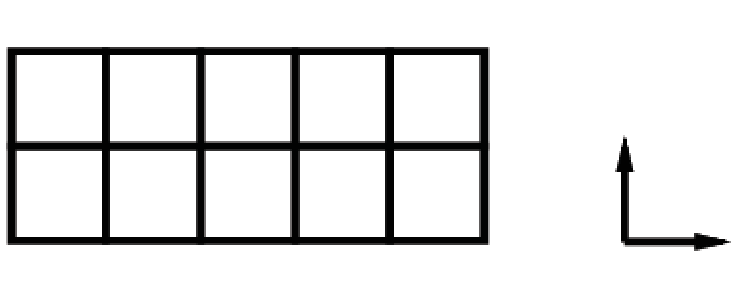
\includegraphics{square-lattice} % requires the graphicx package
   \caption{2D square lattice}
   \label{fig:sqlattice}
\end{figure}
We begin by plotting the trajectories of two runs for two different steps and comparing. As seen in Figures \ref{fig:sqtraj1000} and \ref{fig:sqtraj1e4}, a random walk path for n = 1000 and n = 10,000 steps can take on varying characteristics. In both instances, a random walk is possible in which the tracked position either clusters in several spots or becomes spread out. In both the n = 1000 and n = 10,000 steps, clustering and spreading out behavior is possible. Naturally, the extent of clustering and spreading out scales with the number of steps (i.e., more steps means more clustering or spreading out is possible).

\begin{figure}
\begin{minipage}[htbp]{.49\linewidth}
\centering
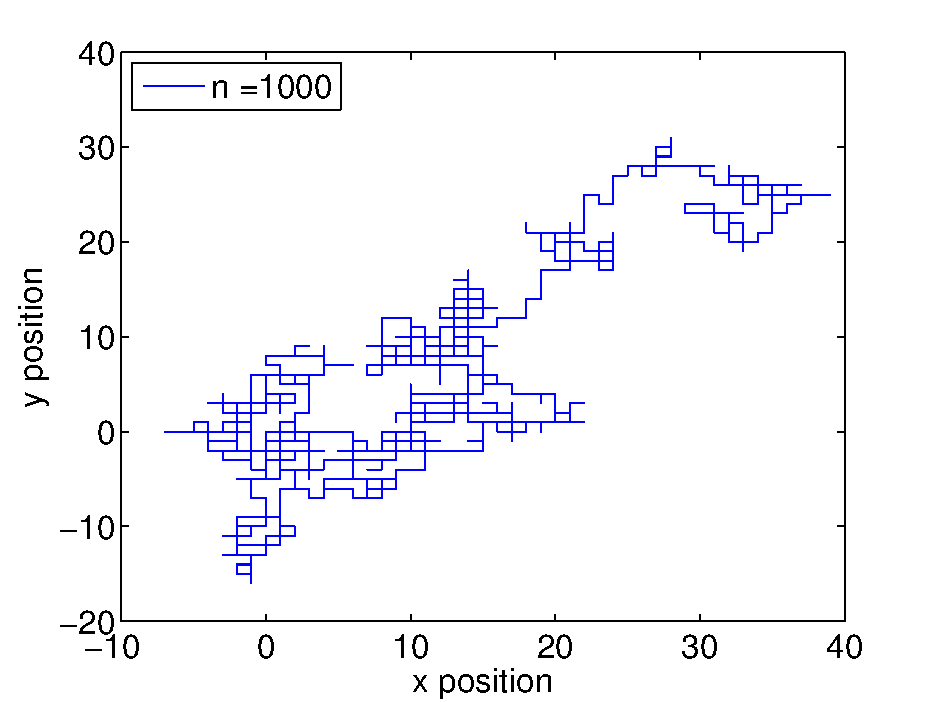
\includegraphics[width=\textwidth]{sqtraj-1000-1}
\end{minipage}
\begin{minipage}[htbp]{.49\linewidth}
\centering
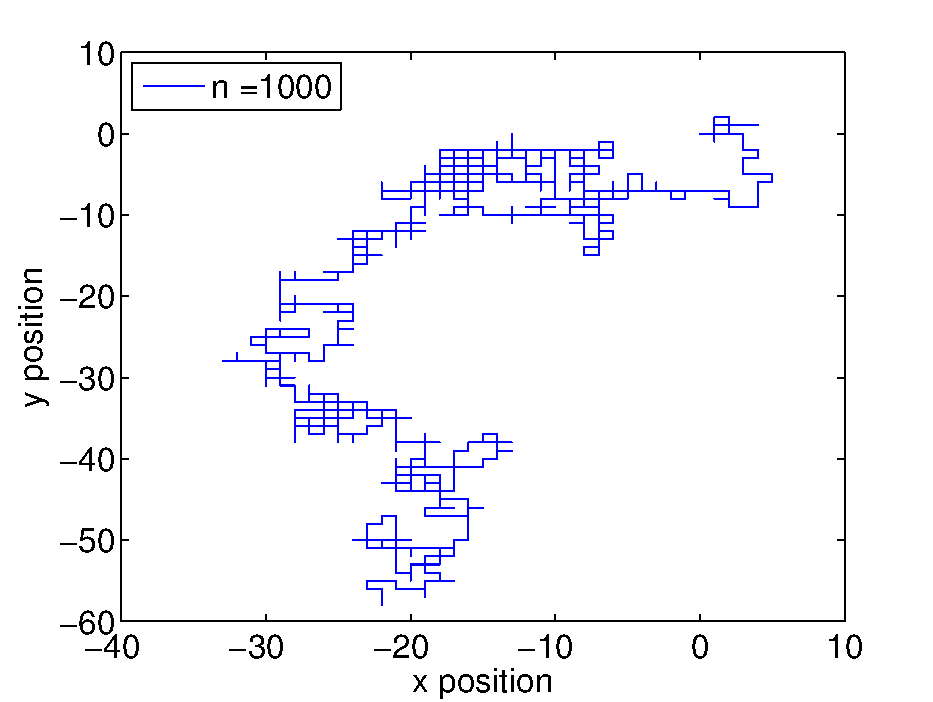
\includegraphics[width=\textwidth]{sqtraj-1000-2}
\end{minipage}
\caption{Sample of trajectories for random walk on 2D square lattice for n = 1000 steps}
\label{fig:sqtraj1000}
\end{figure}

\begin{figure}
\begin{minipage}[htbp]{.49\linewidth}
\centering
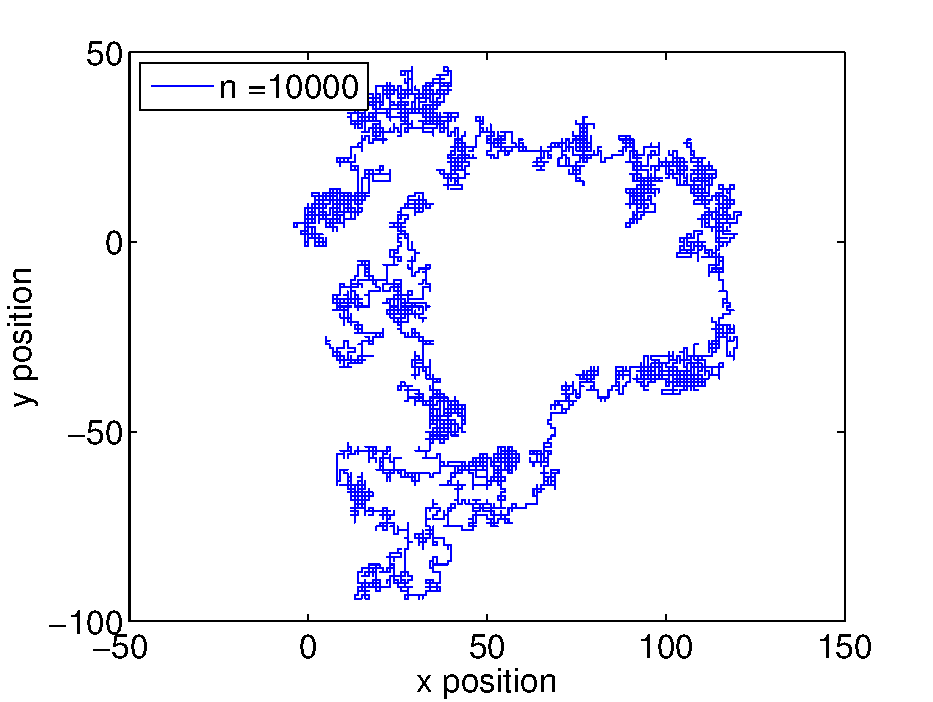
\includegraphics[width=\textwidth]{sqtraj-1e4-1}
\end{minipage}
\begin{minipage}[htbp]{.49\linewidth}
\centering
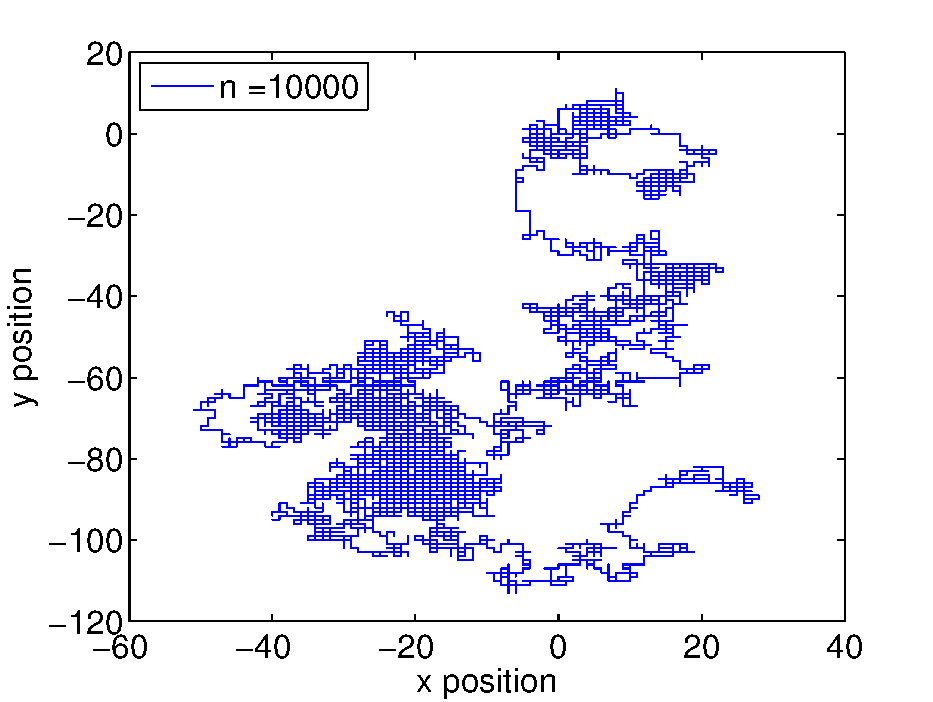
\includegraphics[width=\textwidth]{sqtraj-1e4-2}
\end{minipage}
\caption{Sample of trajectories for random walk on 2D square lattice for n = 10,000 steps}
\label{fig:sqtraj1e4}
\end{figure}

Figure \ref{fig:sqr2} illustrates the mean square distance,$\langle R^2 \rangle$, for a random walker on a 2D square lattice. For $\langle R^2 \rangle$ averaged over a single trajectory, one can observe the jumps where the random walker clusters (i.e., when $\langle R^2 \rangle$ oscillates around a certain value) and where the random walker spreads out or makes a circle (i.e., when $\langle R^2 \rangle$ changes by large amounts). Over the course of several trajectories, the jaggedness of the single trajectory is smoothed out. It takes approximately 100 trajectories to remove major jaggedness and around 250 trajectories to get a curve with reasonable semblance to a straight line; larger numbers of trajectories are shown for reference.

\begin{figure}
\begin{minipage}[htbp]{.49\linewidth}
\centering
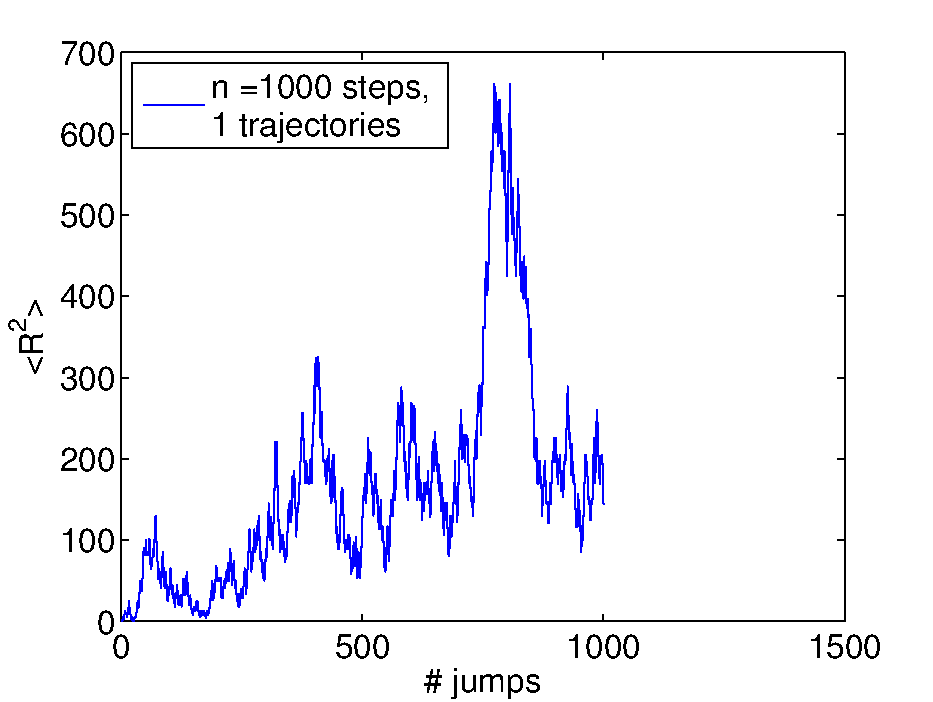
\includegraphics[width=\textwidth]{sqtraj-r2-1}
\end{minipage}
\begin{minipage}[htbp]{.49\linewidth}
\centering
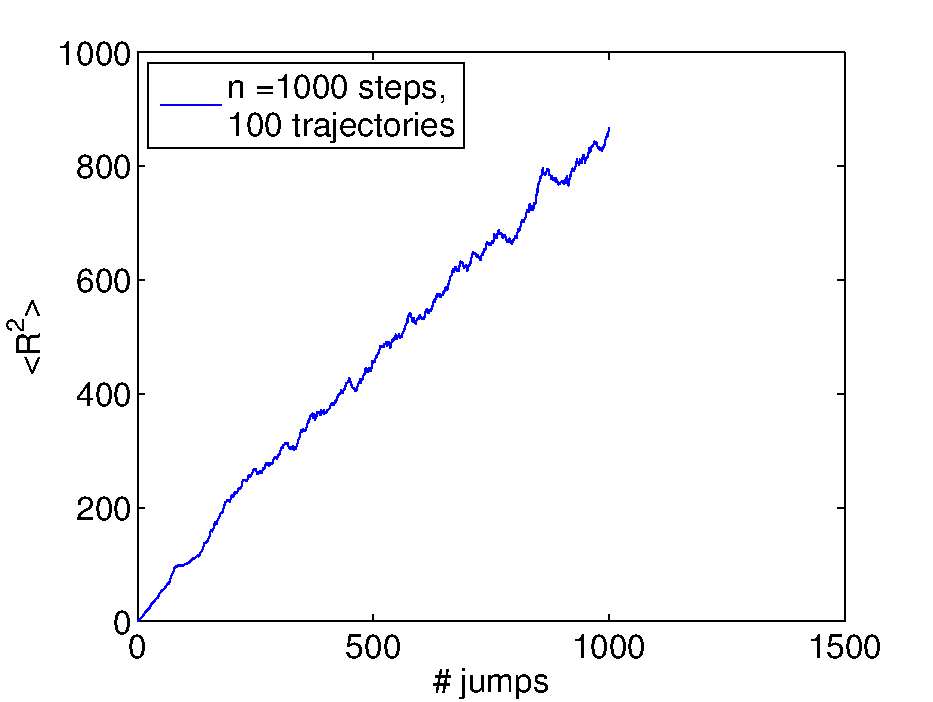
\includegraphics[width=\textwidth]{sqtraj-r2-100}
\end{minipage}
\begin{minipage}[htbp]{.49\linewidth}
\centering
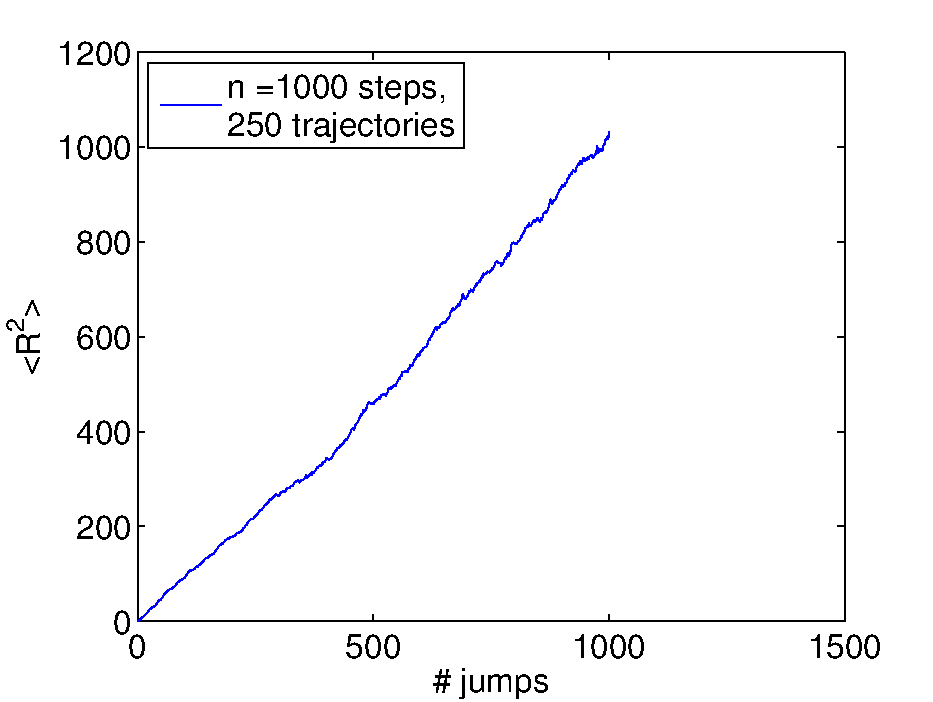
\includegraphics[width=\textwidth]{sqtraj-r2-250}
\end{minipage}
\begin{minipage}[htbp]{.49\linewidth}
\centering
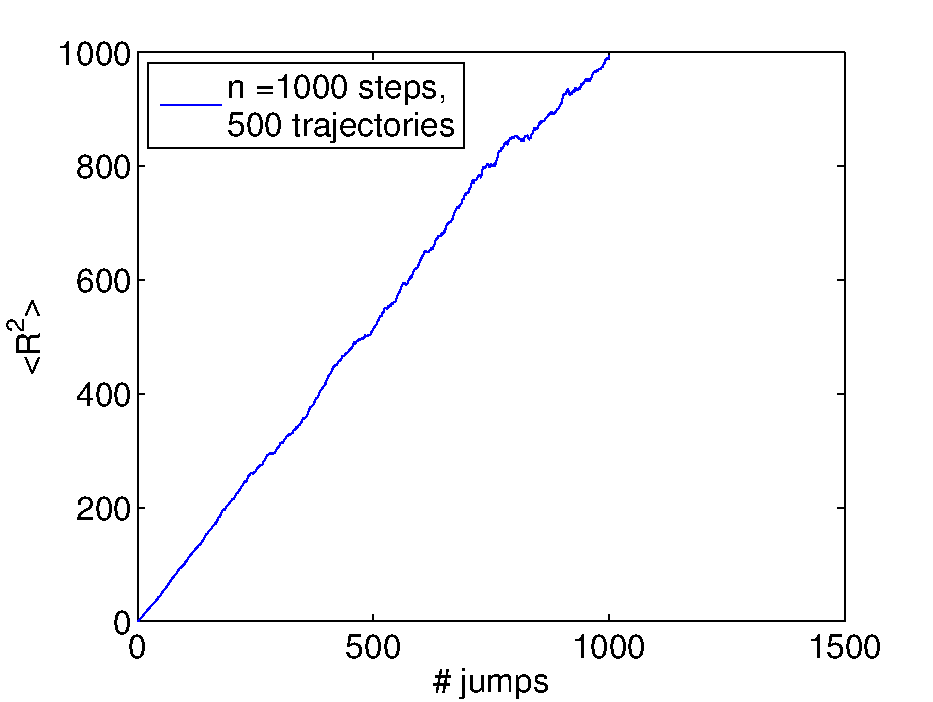
\includegraphics[width=\textwidth]{sqtraj-r2-500}
\end{minipage}
\caption{Mean square distances, $\langle R^2 \rangle$ on 2D square lattice for (a) 1 trajectory (b) 100 trajectories (c) 250 trajectories and (d) 500 trajectories}
\label{fig:sqr2}
\end{figure}
%--------------------------------------------------------------------------------------------------%

\section{Exercise 2: 2D Triangular Lattice}
In a 2D triangular lattice, there are six nearest neighbors. With the initial position at the ???origin, this corresponds to left (-1,0); right(1,0); NE $(\frac{1}{2}, \frac{\sqrt{3}}{2})$; NW $(-\frac{1}{2}, \frac{\sqrt{3}}{2})$; SE $(\frac{1}{2}, -\frac{\sqrt{3}}{2})$ and SW $(-\frac{1}{2}, -\frac{\sqrt{3}}{2})$. Figure \ref{fig:trlattice} shows the basic lattice.

\begin{figure}[htbp]
   \centering
   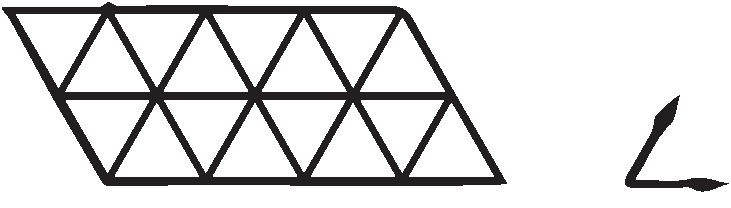
\includegraphics{triangle-lattice} % requires the graphicx package
   \caption{2D triangular lattice}
   \label{fig:trlattice}
\end{figure}

We begin by plotting the trajectories of two runs for two different steps and comparing. As seen in Figures \ref{fig:trtraj1000} and \ref{fig:trtraj1e4}, a random walk path for n = 1000 and n = 10,000 steps can take on varying characteristics, like the 2D square lattice. For the particular runs simulated, in both instances, a random walk is possible in which the tracked position either clusters in several spots or becomes spread out. In both the n = 1000 and n = 10,000 steps, clustering and spreading out behavior is possible. The magnitude of the spread and extent of clustering possible is qualitatively similar to the random walk of the square lattice, but the variation is slightly smaller, possibly due to the triangular lattice have two additional nearest neighbors in comparison. This is also evident in the probability distribution of end-to-end distance discussed for Exercise 5, illustrated in Figure \ref{fig:trbinning}.

\begin{figure}
\begin{minipage}[htbp]{.49\linewidth}
\centering
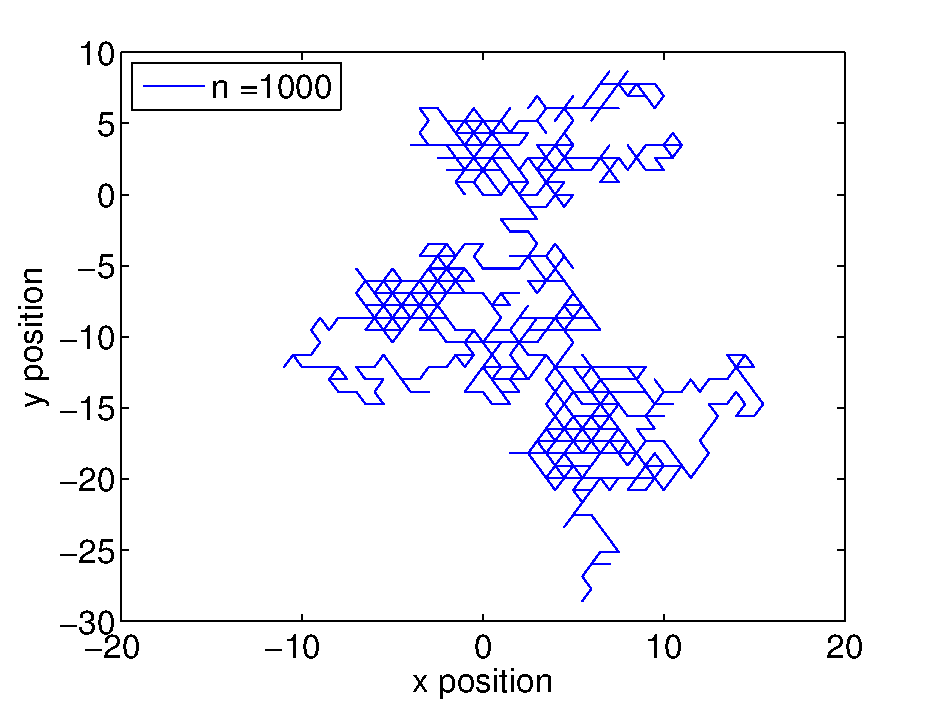
\includegraphics[width=\textwidth]{trtraj-1000-1}
\end{minipage}
\begin{minipage}[htbp]{.49\linewidth}
\centering
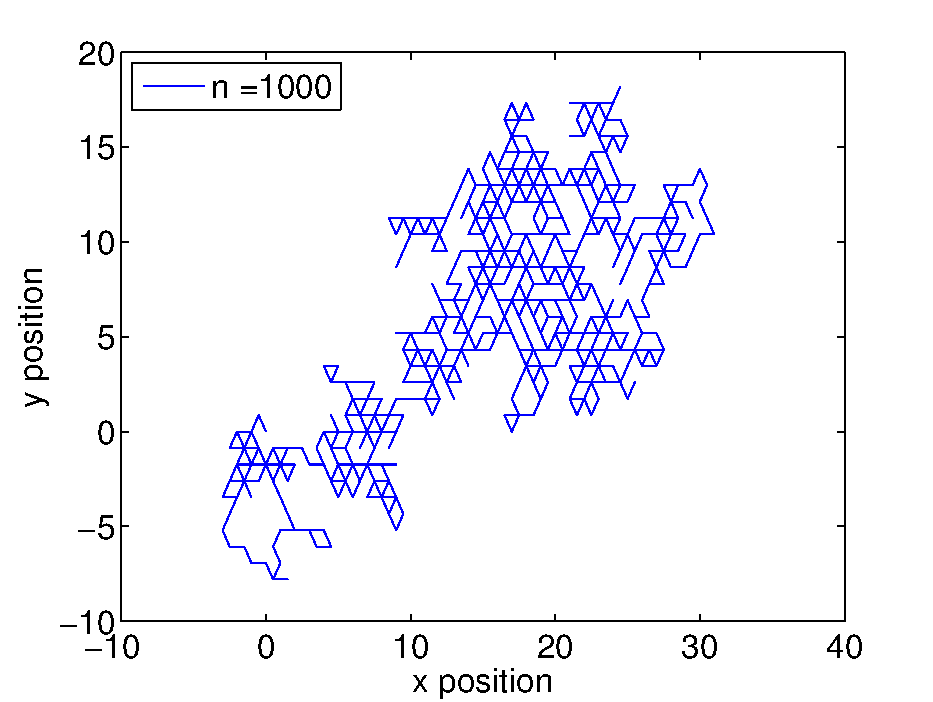
\includegraphics[width=\textwidth]{trtraj-1000-2}
\end{minipage}
\caption{Sample of trajectories for random walk on 2D triangular lattice for n = 1000 steps}
\label{fig:trtraj1000}
\end{figure}

\begin{figure}
\begin{minipage}[htbp]{.49\linewidth}
\centering
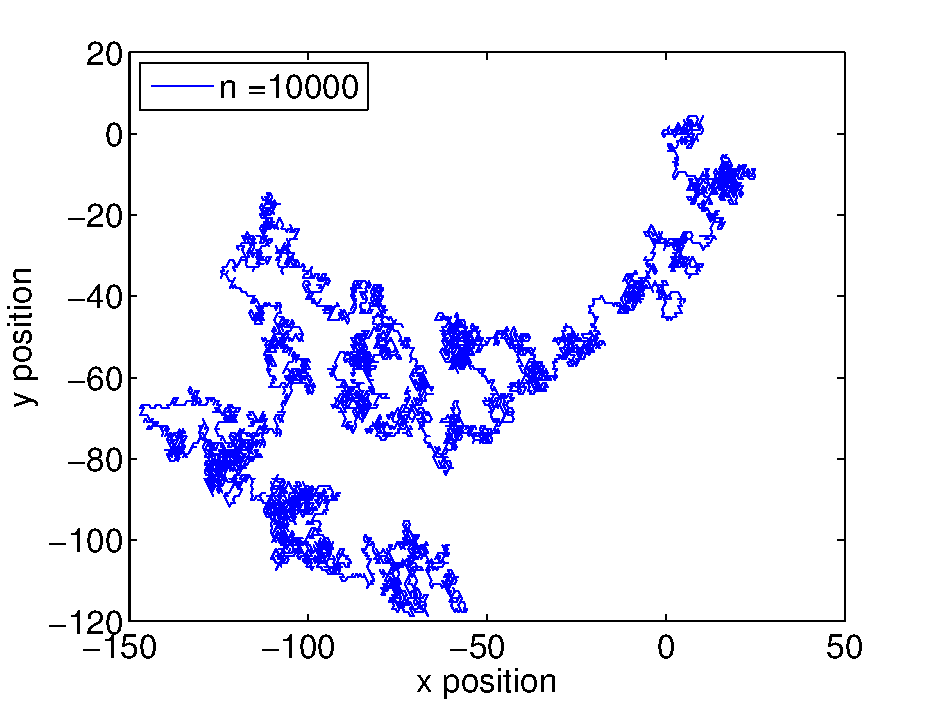
\includegraphics[width=\textwidth]{trtraj-1e4-1}
\end{minipage}
\begin{minipage}[htbp]{.49\linewidth}
\centering
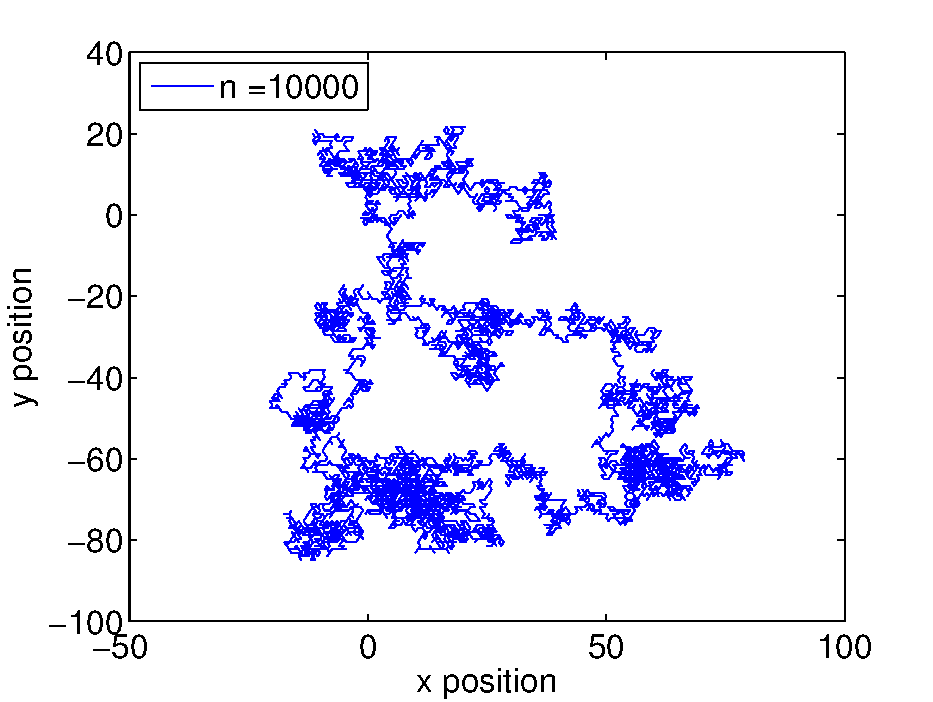
\includegraphics[width=\textwidth]{trtraj-1e4-2}
\end{minipage}
\caption{Sample of trajectories for random walk on 2D triangular lattice for n = 10,000 steps}
\label{fig:trtraj1e4}
\end{figure}

Figure \ref{fig:trr2} illustrates the mean square distance, $\langle R^2 \rangle$, for a random walker on a 2D triangular lattice. Like the square lattice, for $\langle R^2 \rangle$ averaged over a single trajectory, one can observe the jumps where the random walker clusters and spreads out or makes a circle. For the particular trajectory plotted in Figure \ref{fig:trr2}, the random walker followed a path that clustered and eventually made full circle. Over the course of several trajectories, the jaggedness of the single trajectory is smoothed out. It takes approximately 100 trajectories to remove major jaggedness and around 250 trajectories to get a curve with the semblance to a straight line, much like the square lattice; larger numbers of trajectories are shown for reference.

\begin{figure}
\begin{minipage}[htbp]{.49\linewidth}
\centering
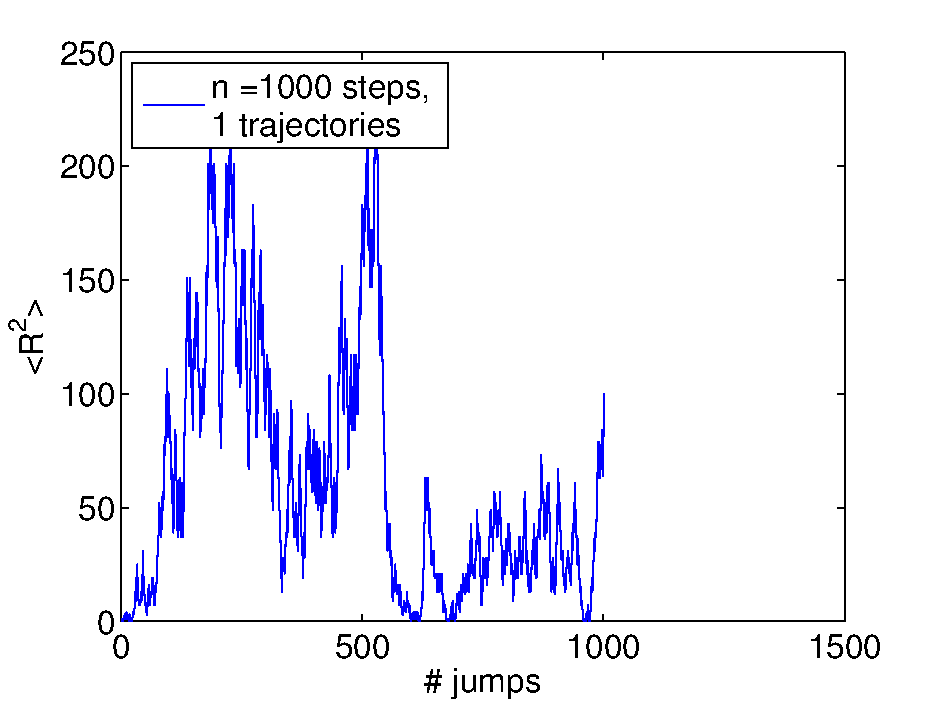
\includegraphics[width=\textwidth]{trtraj-r2-1}
\end{minipage}
\begin{minipage}[htbp]{.49\linewidth}
\centering
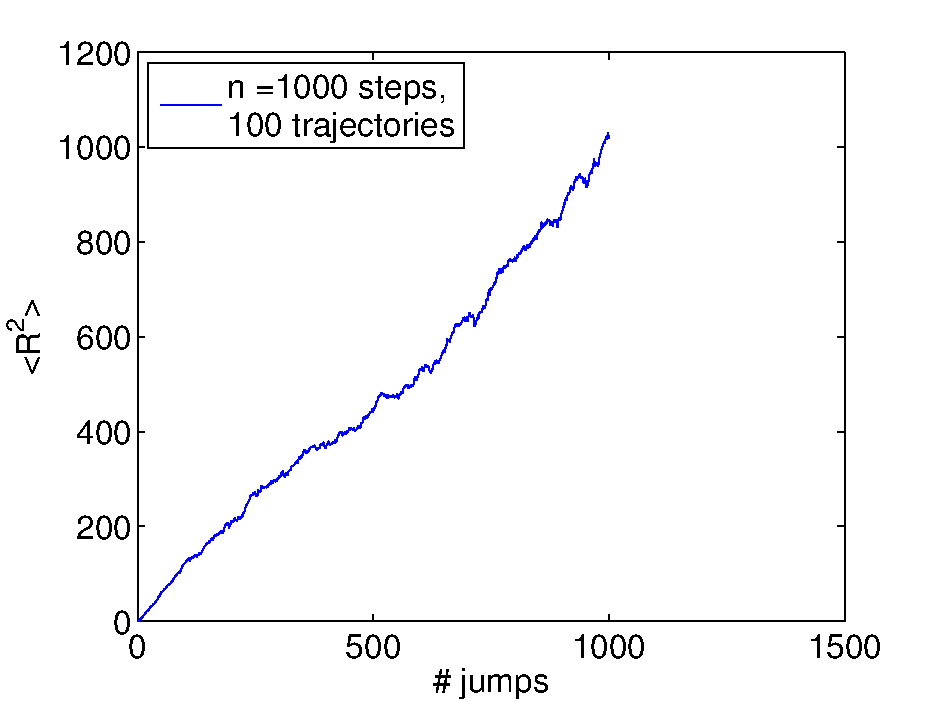
\includegraphics[width=\textwidth]{trtraj-r2-100}
\end{minipage}
\begin{minipage}[htbp]{.49\linewidth}
\centering
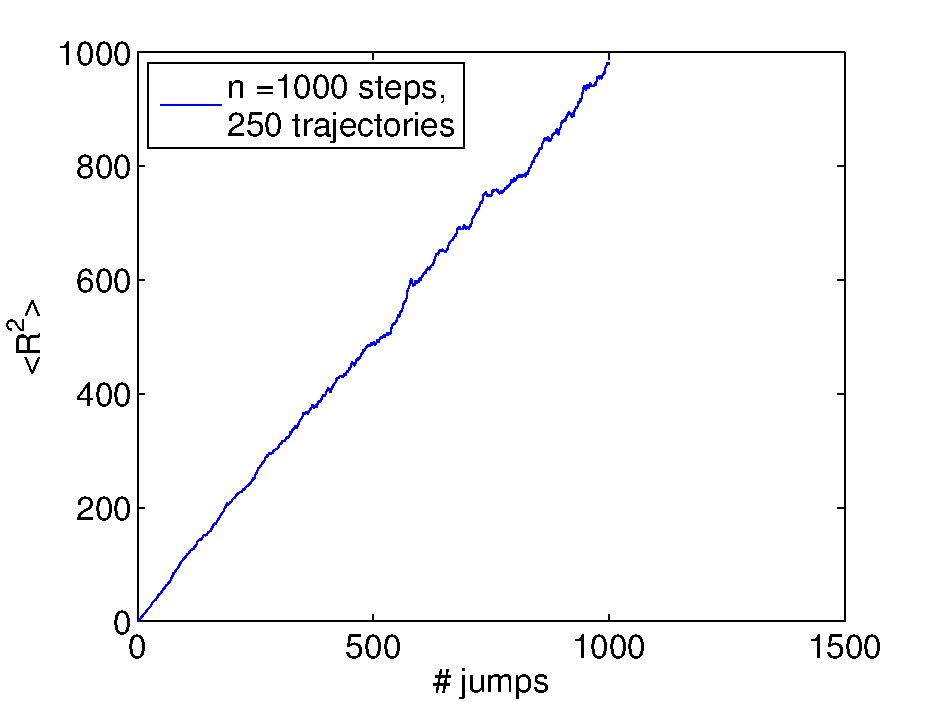
\includegraphics[width=\textwidth]{trtraj-r2-250}
\end{minipage}
\begin{minipage}[htbp]{.49\linewidth}
\centering
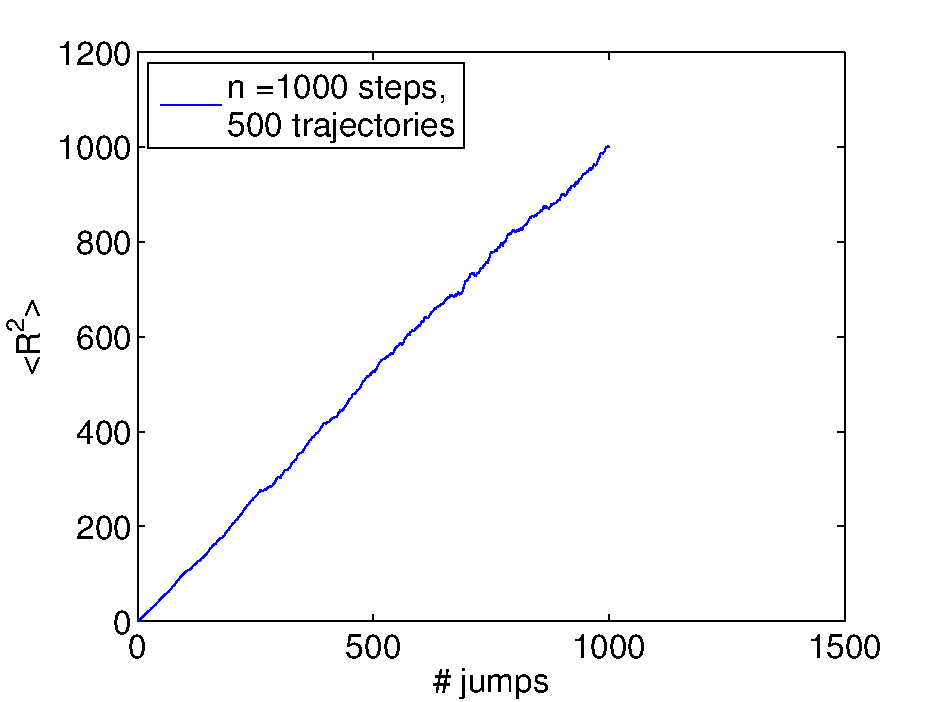
\includegraphics[width=\textwidth]{trtraj-r2-500}
\end{minipage}
\caption{Mean square distances, $\langle R^2 \rangle$ on 2D triangular lattice for (a) 1 trajectory (b) 100 trajectories (c) 250 trajectories and (d) 500 trajectories}
\label{fig:trr2}
\end{figure}

%--------------------------------------------------------------------------------------------------%
\section{Exercise 3: 3D Simple Cubic Lattice}

In a 3D cubic lattice, there are six nearest neighbors. With the initial position at the origin, this corresponds to left (-1,0,0); right(1,0,0); in (0,1,0); out (0,-1,0); up (0,0,1); and down (0,0,-1). We implement a similar procedure for 3D paths much like the 2D square and triangular lattices. For the samples of trajectories plotted in Figures \ref{fig:cubtraj1000} and \ref{fig:cubtraj1e4}, the similar range of random walk paths of clustering and spreading is observed. Surprisingly, despite the added degree of freedom in the third dimension, the range of spread for the random walker on the 3D cubic lattice is of similar ranges to the square and more so the triangular lattice when considering the range along a single axis. This may be reflected in the fact that the number of nearest neighbors for the cubic lattice is equal to that of the triangular lattice and comparable to that of the square lattice, and so effectively have similar degrees of freedom. A similar behavior is observed between n = 1000 and n = 10,000 step trajectories, as found in the square and triangular lattice.

\begin{figure}
\begin{minipage}[htbp]{.49\linewidth}
\centering
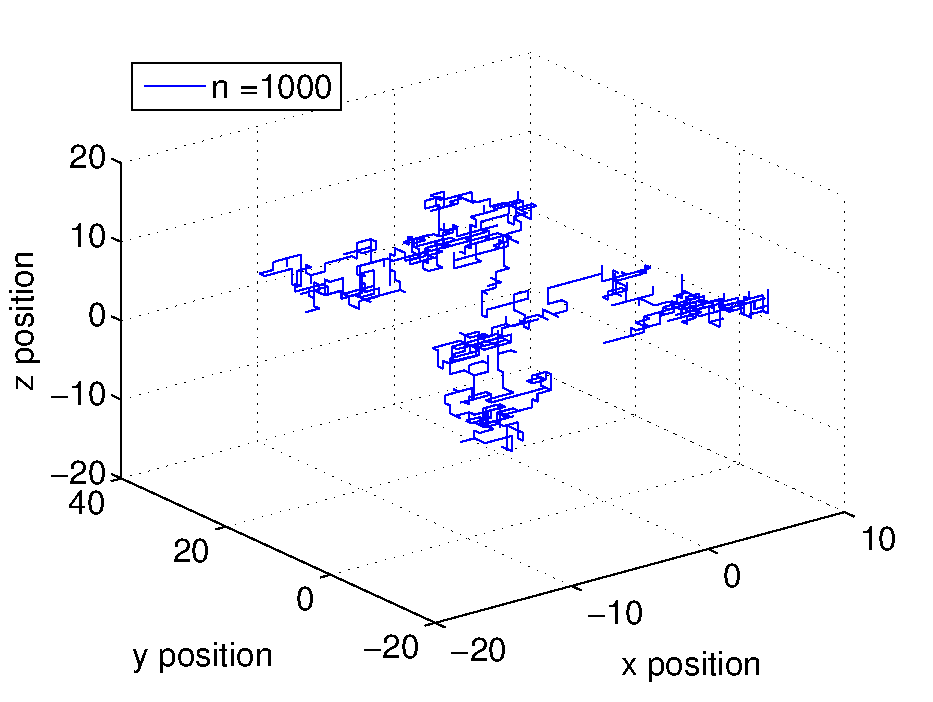
\includegraphics[width=\textwidth]{cub-traj-1000-1}
\end{minipage}
\begin{minipage}[htbp]{.49\linewidth}
\centering
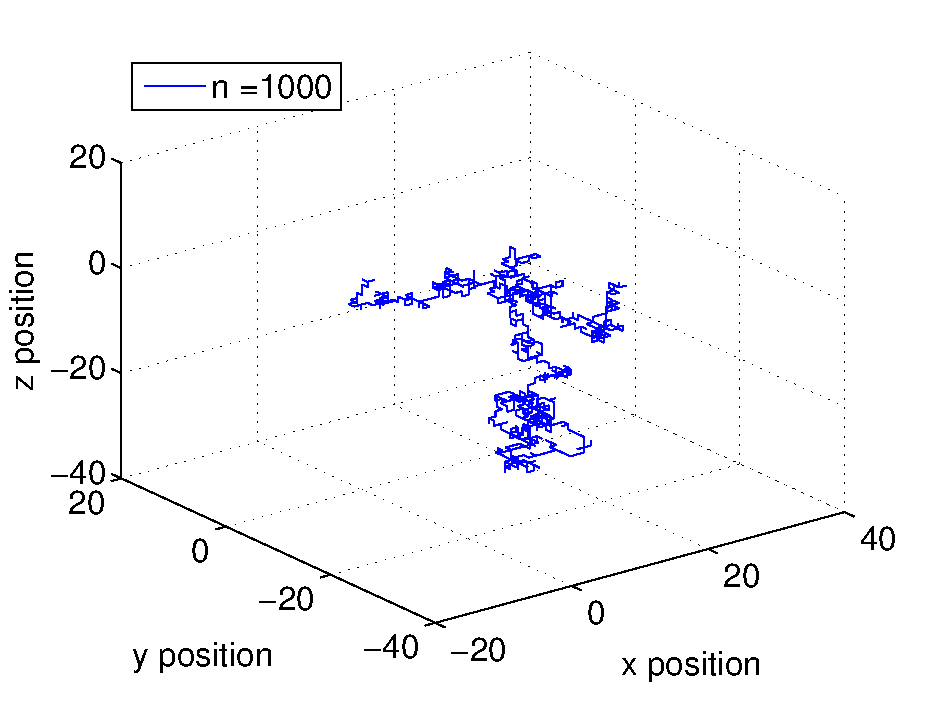
\includegraphics[width=\textwidth]{cub-traj-1000-2}
\end{minipage}
\caption{Sample of trajectories for random walk on 3D cubic lattice for n = 1000 steps}
\label{fig:cubtraj1000}
\end{figure}

\begin{figure}
\begin{minipage}[htbp]{.49\linewidth}
\centering
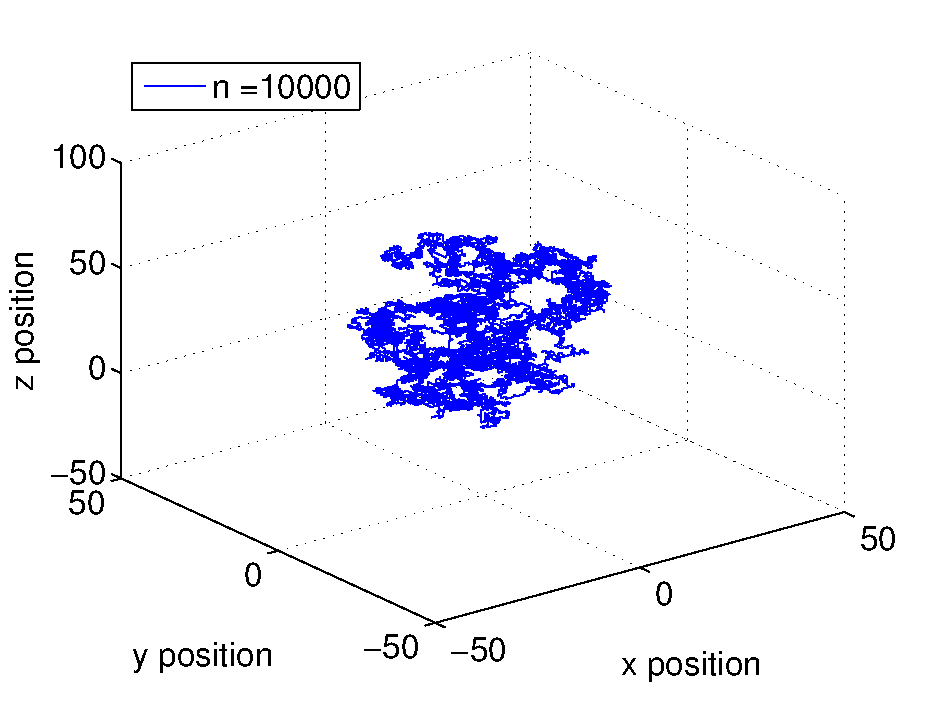
\includegraphics[width=\textwidth]{cub-traj-1e4-1}
\end{minipage}
\begin{minipage}[htbp]{.49\linewidth}
\centering
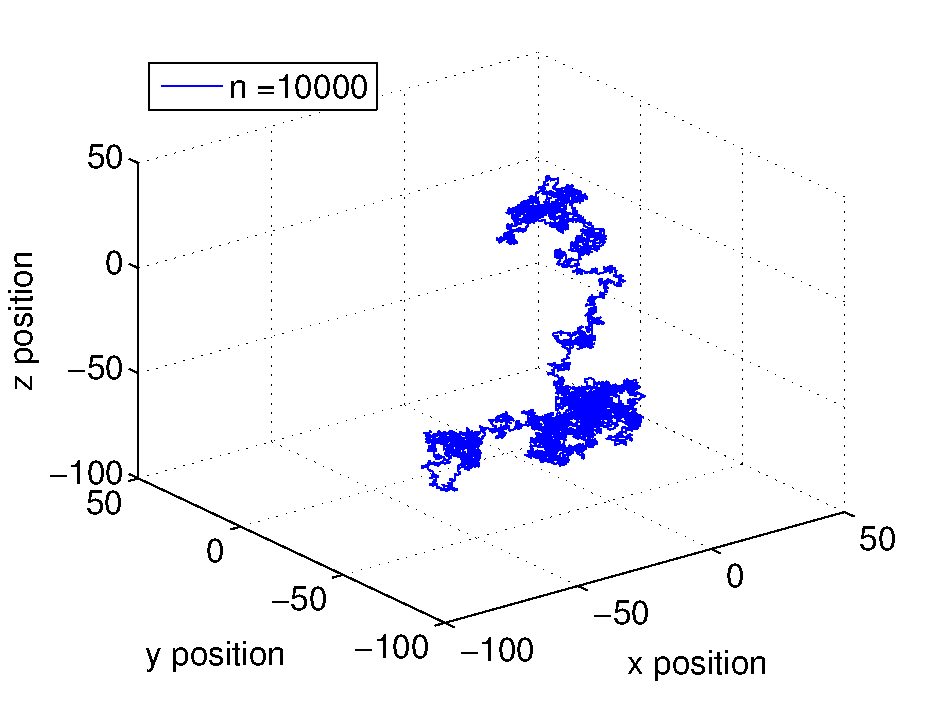
\includegraphics[width=\textwidth]{cub-traj-1e4-2}
\end{minipage}
\caption{Sample of trajectories for random walk on 3D cubic lattice for n = 10,000 steps}
\label{fig:cubtraj1e4}
\end{figure}

The similarity of average spread that is possible in the cubic lattice compared to the square and triangular lattice is apparent in the $\langle R^2 \rangle$ curves, in which the observed $\langle R^2 \rangle$ averaged over many trajectories is similar, if not the same. Similar conclusions can thus be made about the cubic lattice that have been made for the square and triangular lattices. Similarly, it takes about 200 trajectories for $\langle R^2 \rangle$ to even out to a straight line, which is (arbitrarily to a certain extent) smaller than that of the square and triangular lattice.

\begin{figure}
\begin{minipage}[htbp]{.49\linewidth}
\centering
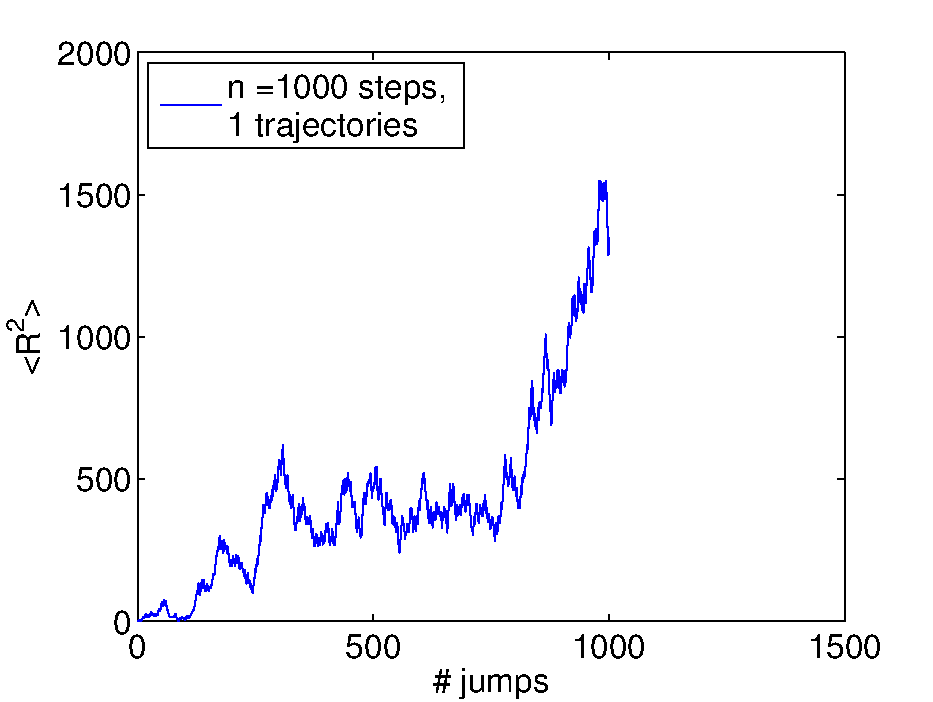
\includegraphics[width=\textwidth]{cub-r2-1}
\end{minipage}
\begin{minipage}[htbp]{.49\linewidth}
\centering
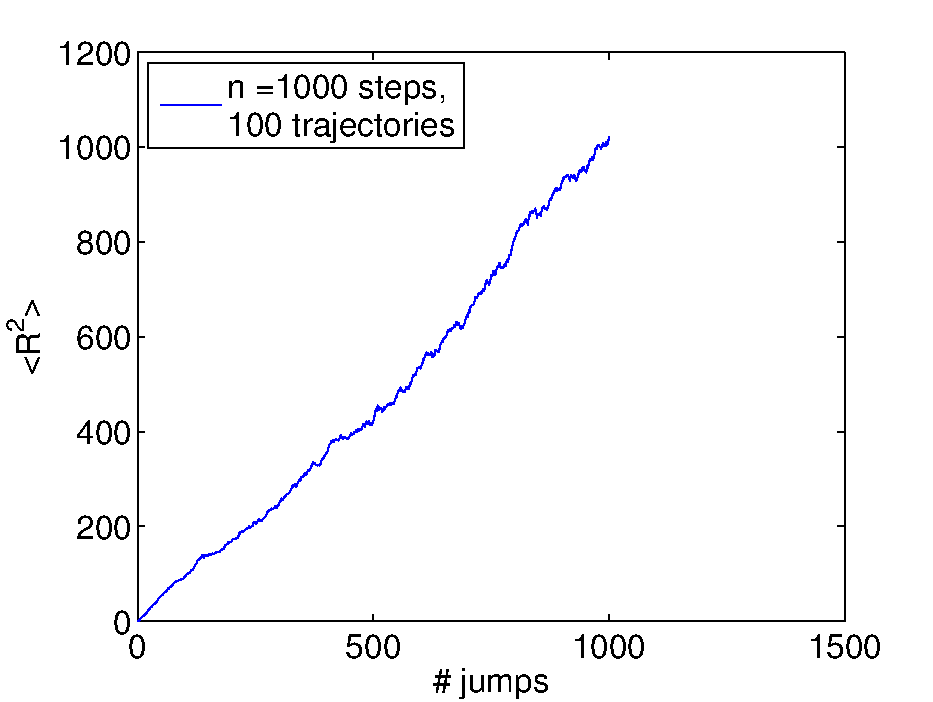
\includegraphics[width=\textwidth]{cub-r2-100}
\end{minipage}
\begin{minipage}[htbp]{.49\linewidth}
\centering
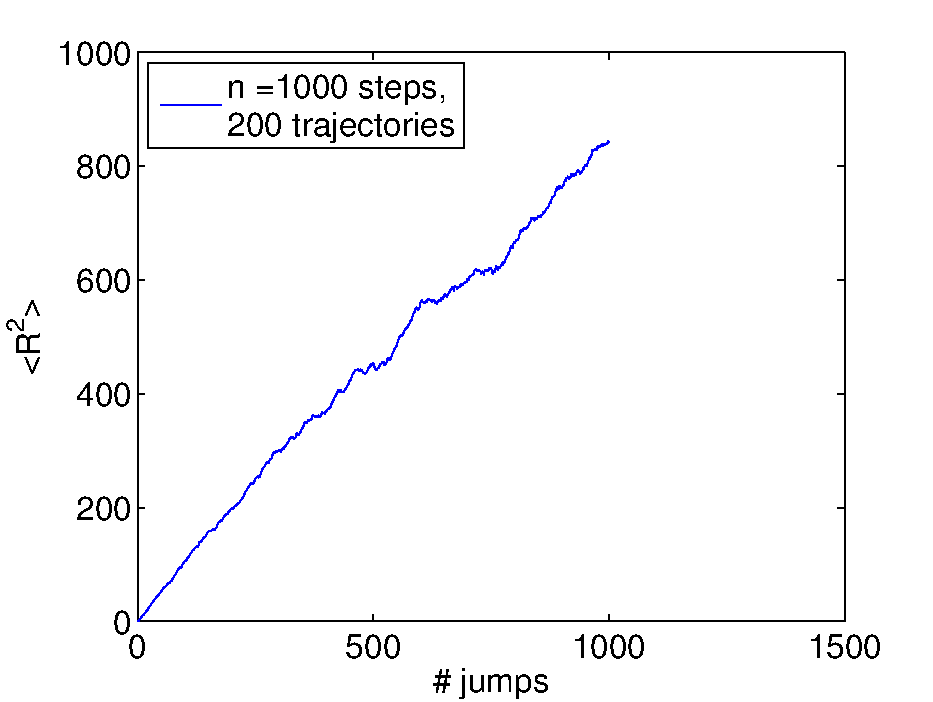
\includegraphics[width=\textwidth]{cub-r2-200}
\end{minipage}
\begin{minipage}[htbp]{.49\linewidth}
\centering
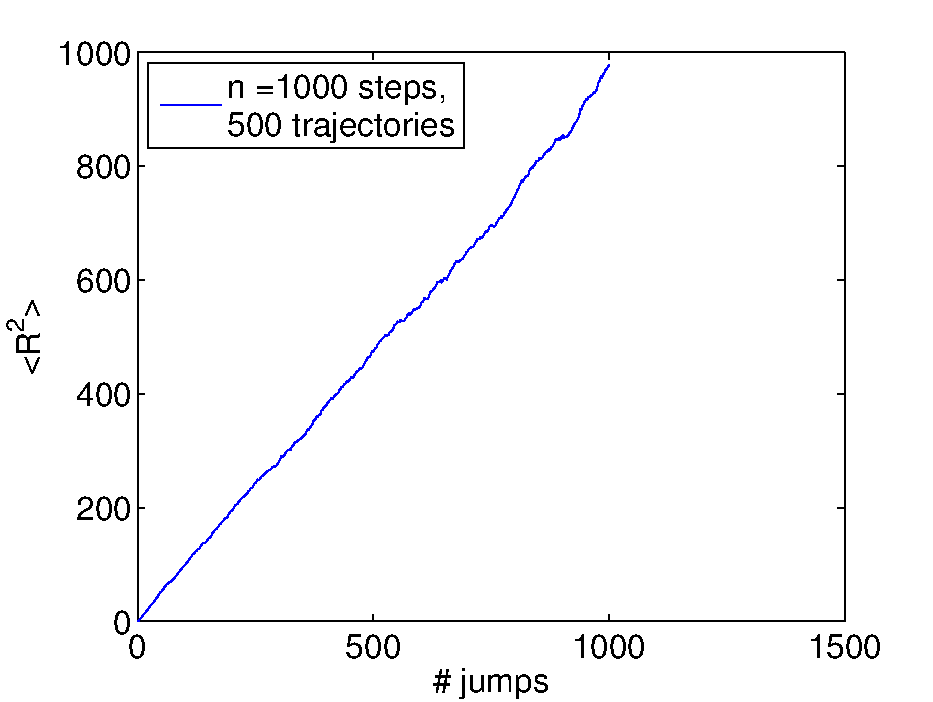
\includegraphics[width=\textwidth]{cub-r2-500}
\end{minipage}
\caption{Mean square distances, $<R^{2}>$ on 3D cubic lattice for (a) 1 trajectory (b) 100 trajectories (c) 200 trajectories and (d) 500 trajectories}
\label{fig:cubr2}
\end{figure}

Overall, as illustrated in Figure \ref{fig:cubbinning}, the averaged behavior of random walk in the cubic lattice has less spread and path variation (i.e., smaller peak and similar but slightly smaller peak width). The cubic lattice thus tends to favor extreme clustering and spread less than the square lattice. As illustrated in Figure \ref{fig:cubbinning}, the probability distribution between the cubic and triangular lattice is similar, despite their different dimensionality. This once again suggests that this may be due to the fact that the cubic and triangular lattice both have 6 nearest neighbors, and thus similar degrees of freedom. A major difference is that the triangular lattice favors extreme clustering more (i.e., higher probabilities for small $R_{N}$ ).

%--------------------------------------------------------------------------------------------------%
\section{Exercise 4: 3D FCC Lattice}

In a 3D FCC lattice, there are twelve nearest neighbors. With the initial position at the origin, for \textit{a} = 1, this corresponds to

\begin{multicols}{2}
 \begin{enumerate}
   \item $(\frac{1}{2}, \frac{1}{2}, 0)$
   \item $(\frac{1}{2}, -\frac{1}{2}, 0)$
   \item $(\frac{1}{2}, 0, \frac{1}{2})$
   \item $(\frac{1}{2}, 0, -\frac{1}{2})$
   \item $(-\frac{1}{2}, -\frac{1}{2}, 0)$
   \item $(-\frac{1}{2}, \frac{1}{2}, 0)$
   \item $(-\frac{1}{2}, 0, -\frac{1}{2})$
   \item $(-\frac{1}{2}, 0, \frac{1}{2})$
   \item $(0, \frac{1}{2}, -\frac{1}{2})$
   \item $(0, \frac{1}{2}, \frac{1}{2})$
   \item $(0, -\frac{1}{2}, -\frac{1}{2})$
   \item $(0, -\frac{1}{2}, \frac{1}{2})$
 \end{enumerate}
 \end{multicols}{2}
 
 We begin by plotting the trajectories of two runs for two different steps and comparing. As observed in Figures \ref{fig:fcctraj1000} and \ref{fig:fcctraj1e4}, a spread and clustering behavior is also observed. However, unlike the previous lattices investigated, there is substantially more clustering that occurs for several tests of trajectories. This is apparent when comparing the range of spread of a sample of possible trajectories, which is on the order of the square lattice, for both the n = 1000 and n = 10,000 step trajectories, which is unlike the square, triangular, and cubic lattice where more steps results in large spread.

\begin{figure}
\begin{minipage}[htbp]{.49\linewidth}
\centering
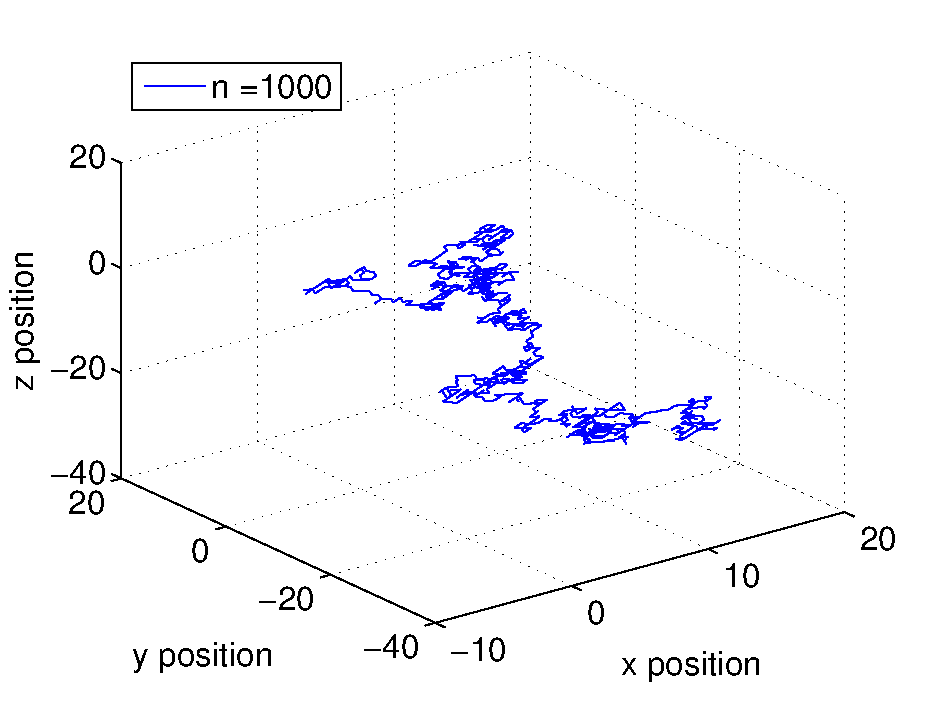
\includegraphics[width=\textwidth]{fcc-traj-1000-1}
\end{minipage}
\begin{minipage}[htbp]{.49\linewidth}
\centering
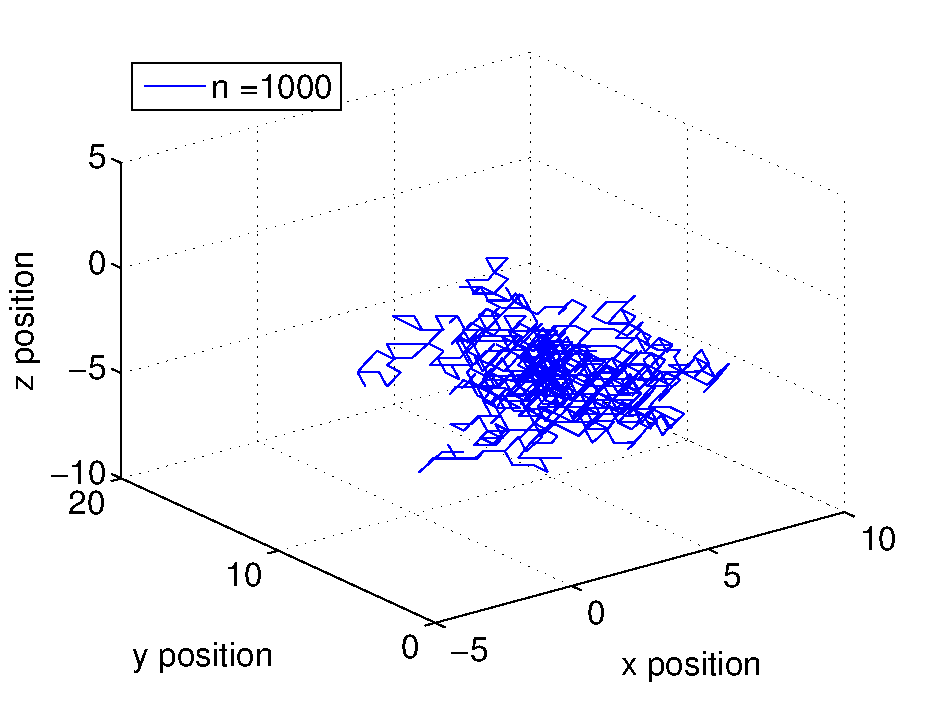
\includegraphics[width=\textwidth]{fcc-traj-1000-2}
\end{minipage}
\caption{Sample of trajectories for random walk on 3D FCC lattice for n = 1000 steps}
\label{fig:fcctraj1000}
\end{figure}

\begin{figure}
\begin{minipage}[htbp]{.49\linewidth}
\centering
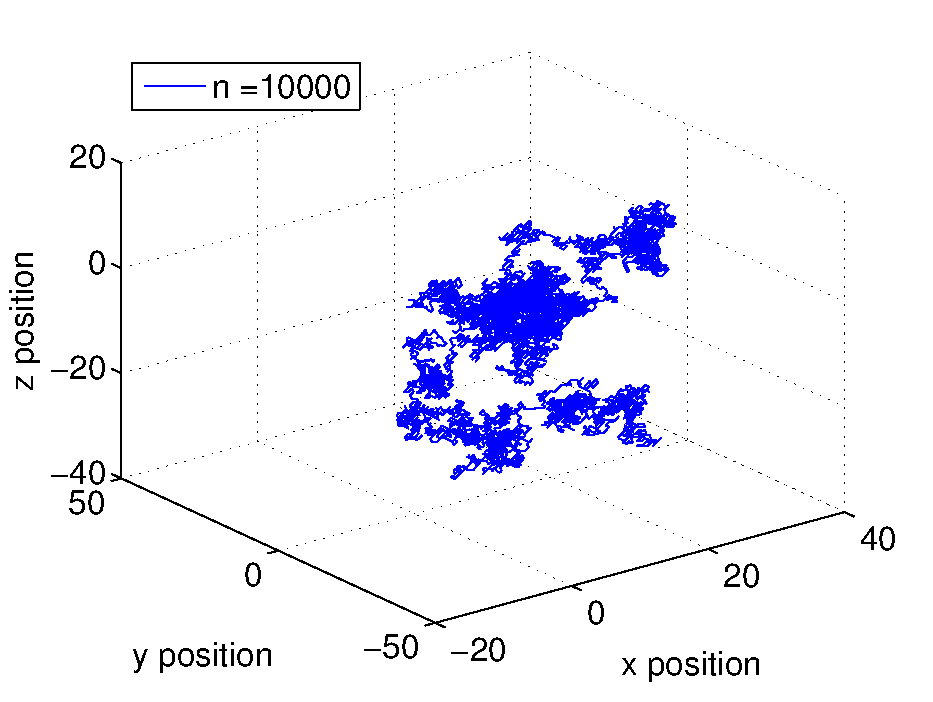
\includegraphics[width=\textwidth]{fcc-traj-1e4-1}
\end{minipage}
\begin{minipage}[htbp]{.49\linewidth}
\centering
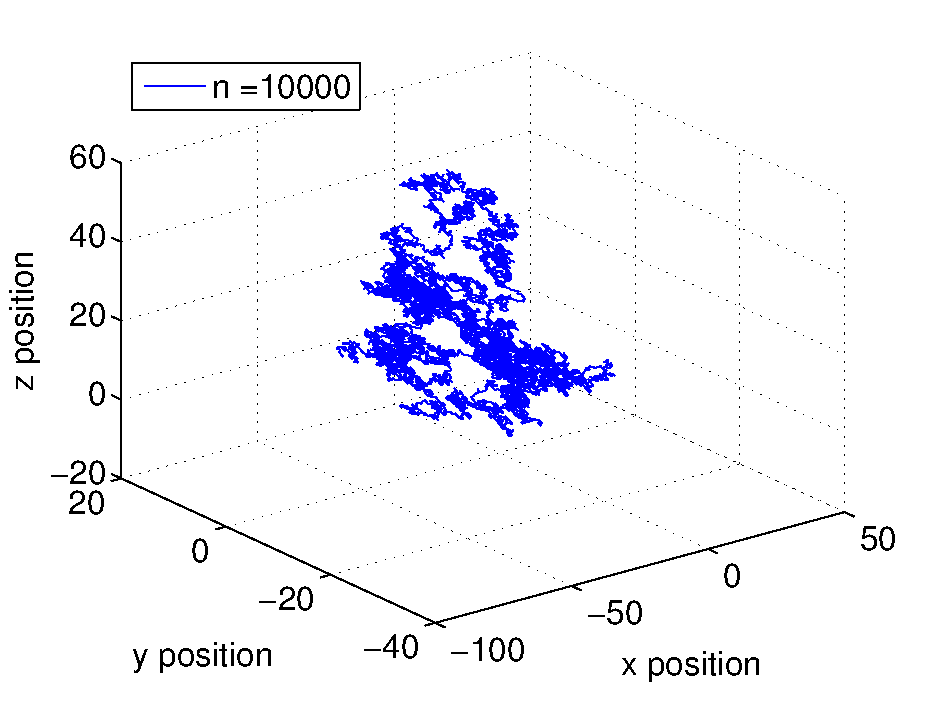
\includegraphics[width=\textwidth]{fcc-traj-1e4-2}
\end{minipage}
\caption{Sample of trajectories for random walk on 3D FCC lattice for n = 10,000 steps}
\label{fig:fcctraj1e4}
\end{figure}

This pronounced clustering behavior is also evident in tracking the $\langle R^2 \rangle$ behavior, which is nearly half that of the other lattices, though it smooths out for around the same number of trajectories averaged over. This may be due to the fact that for any atom in the FCC lattice, there are twelve nearest neighbors, meaning random walk has more opportunities to not diffuse through the lattice. This is analogous to the general scaling of diffusivity with the inverse of the dimensionality; in that increased dimensionality (i.e., degrees of freedom) results in decreased diffusivity. Yet it takes on the order of 150 trajectories to average out the jaggedness of the mean square distance, much smaller than that of the other lattices tested, that suggests less spread. The increased amounts of clustering is particularly evident in the narrowing and shift of the peak in the probability distribution of end-to-end distance, as shown in Figure \ref{fig:fccbinning}.

\begin{figure}
\begin{minipage}[htbp]{.49\linewidth}
\centering
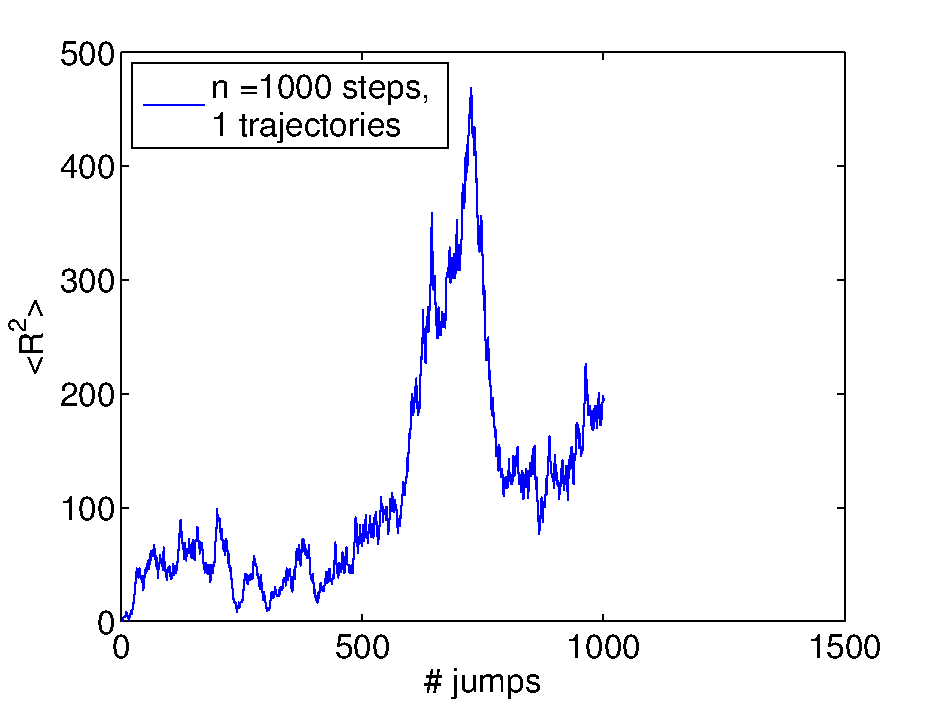
\includegraphics[width=\textwidth]{fcc-r2-1}
\end{minipage}
\begin{minipage}[htbp]{.49\linewidth}
\centering
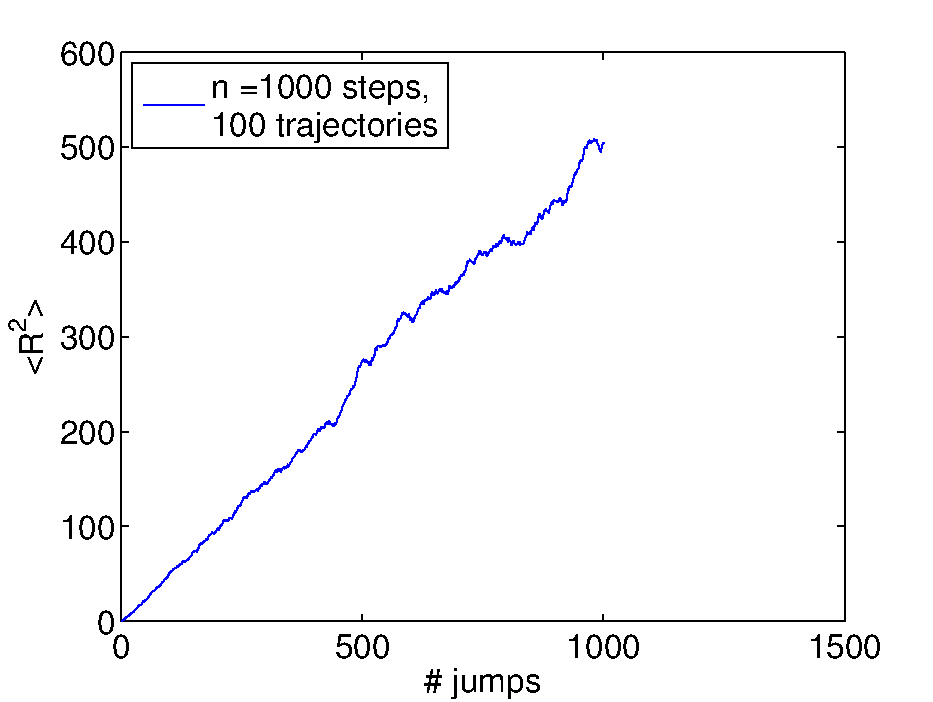
\includegraphics[width=\textwidth]{fcc-r2-100}
\end{minipage}
\begin{minipage}[htbp]{.49\linewidth}
\centering
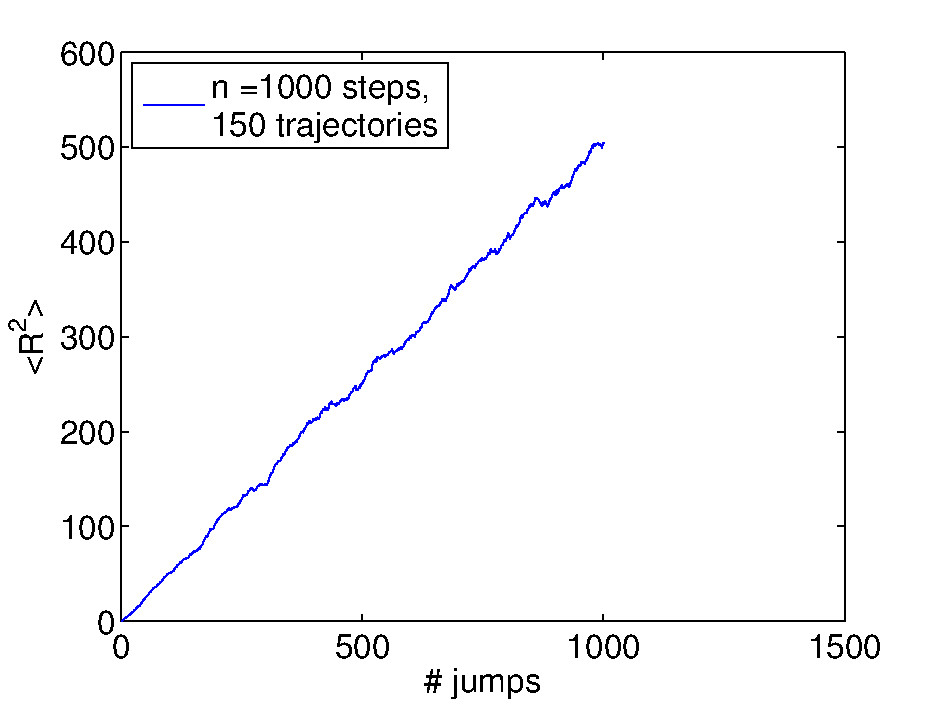
\includegraphics[width=\textwidth]{fcc-r2-150}
\end{minipage}
\begin{minipage}[htbp]{.49\linewidth}
\centering
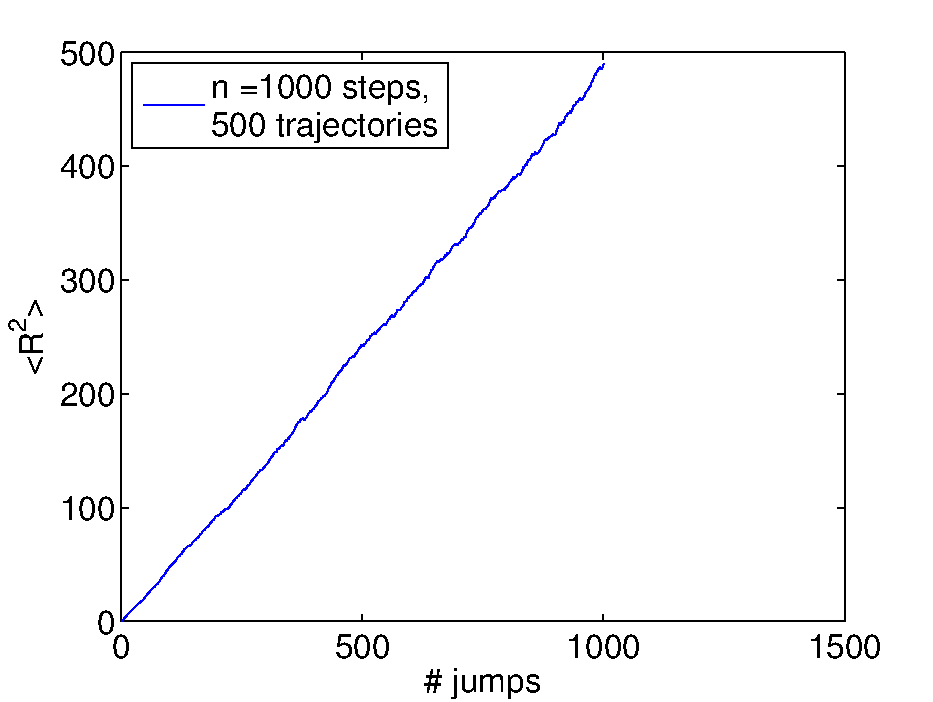
\includegraphics[width=\textwidth]{fcc-r2-500}
\end{minipage}
\caption{Mean square distances, $\langle R^2 \rangle$ on 3D FCC lattice for (a) 1 trajectory (b) 100 trajectories (c) 150 trajectories and (d) 500 trajectories}
\label{fig:fccr2}
\end{figure}

%--------------------------------------------------------------------------------------------------%
\section{Exercise 5: Binning for Probability Distribution of end-to-end distance}

Attached with this document is the binning procedure used to create the following histograms. The basic idea is to divide the simulated end-to-end distances into bins demarcated by equally spaced intervals, counting the frequency of distances that fall within the specified range. In addition to the probabilities, one must also account for the normalization factor introduced by varying the number of bins, as the integrated probability of the probability distribution must sum to unity.
Below are plots that compare the probability distribution of end-to-end distances simulated for the four lattices examined earlier, in comparison to the predicted curve provided in LeSar. Since the analytical version for the cubic lattice is readily available, it is used as the reference for comparison. Figure \ref{fig:cubbinning} provides a comparison between model and simulation, illustrating that within reasonable statistical variation, the model describes well random walk behavior on a cubic lattice.

We plot this same probability distribution function in comparison to the triangular lattice in Figure \ref{fig:trbinning}. Figure \ref{fig:sqbinning} illustrates from a different perspective what the plotted trajectories and $\langle R^2 \rangle$ plots showed qualitatively; that the spread of random walks in the square and cubic lattice are similar, though in the square lattice, there is not as much spread possible (i.e., smaller and narrower peak) and possibly less clustering in general (i.e., less frequency in smaller end-to-end distances). A similar conclusion can be made about the triangular lattice, from Figure \ref{fig:trbinning}. The lattice with greatest difference in random walk behavior is once again the FCC lattice, as evidenced in Figure \ref{fig:fccbinning}. Not only is the peak narrower, but it is shifted to favor smaller end-to-end distances, indicating increased clustering and less spread, which were observed from the previously plotted trajectories and $\langle R^2 \rangle$ behaviors.

 \begin{figure}[htbp]
    \centering
    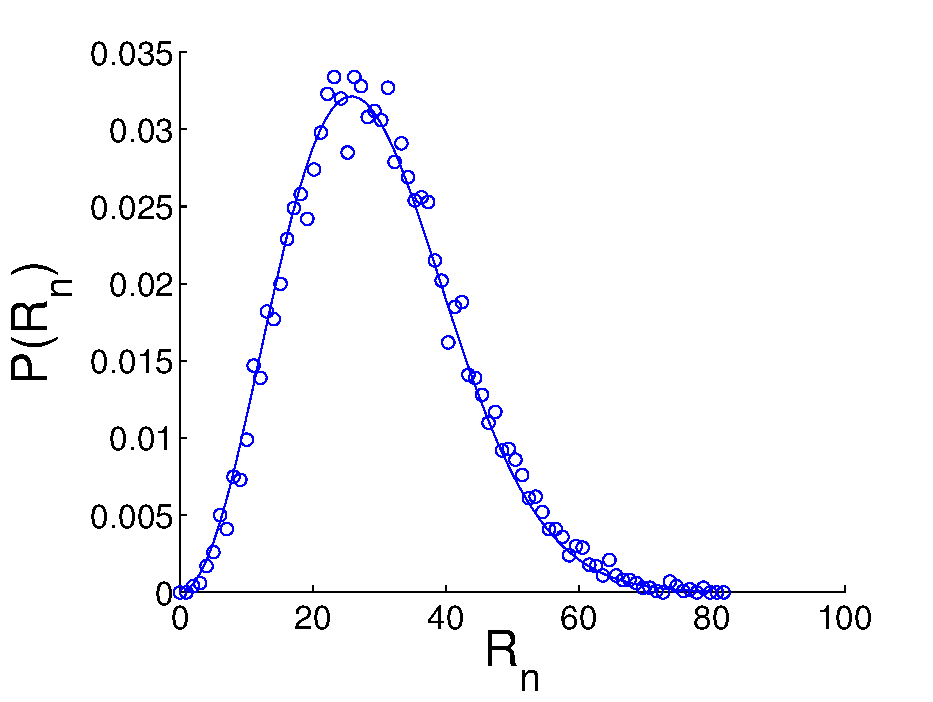
\includegraphics{binning-cub-1000n-10ktr-80bin} % requires the graphicx package
    \caption{Probability distribution of simulated end-to-end distances for random walk in cubic lattice (empty circles) plotted against that of cubic lattice for comparison between theory and simulation; done for n = 1000 steps, 10k trials, and 80 bins (solid line)}
    \label{fig:cubbinning}
 \end{figure}

\begin{figure}[htbp]
   \centering
   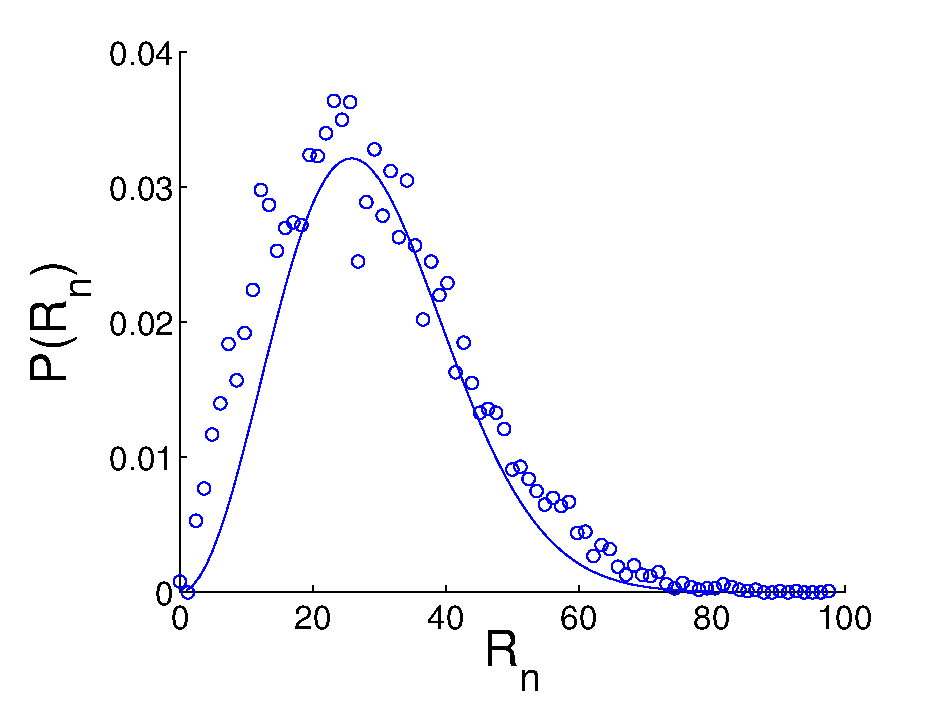
\includegraphics{binning-sq-1000n-10ktr-80bin} % requires the graphicx package
   \caption{Probability distribution of simulated end-to-end distances for random walk in square lattice (empty circles) plotted against that of cubic lattice for comparison in clustering and spread behavior; done for n = 1000 steps, 10k trials, and 80 bins (solid line)}
   \label{fig:sqbinning}
\end{figure}

\begin{figure}[htbp]
   \centering
   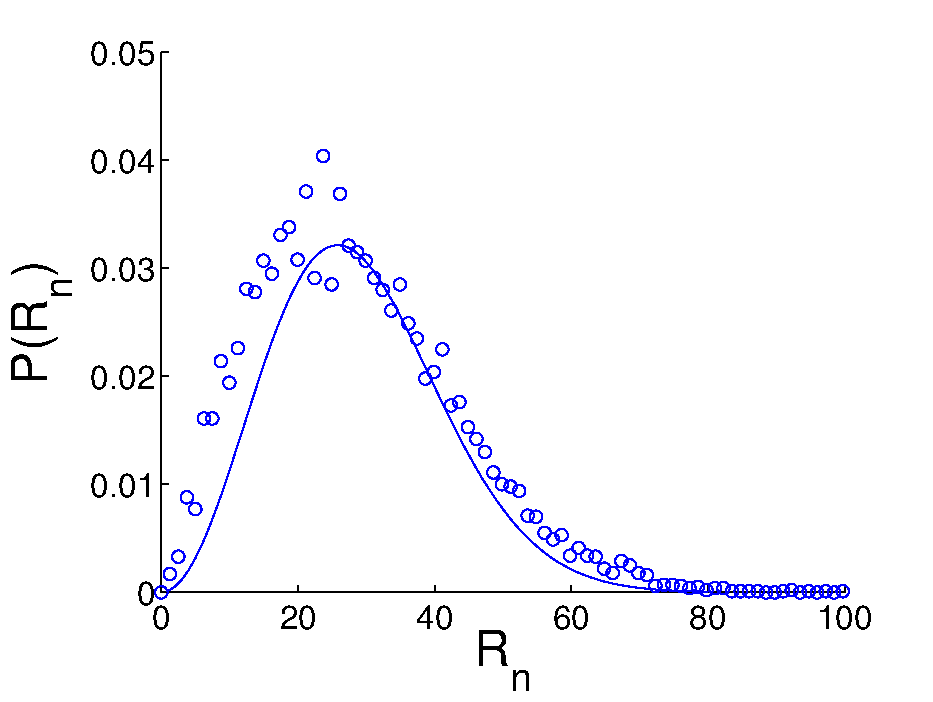
\includegraphics{binning-tr-1000n-10ktr-80bin} % requires the graphicx package
   \caption{Probability distribution of simulated end-to-end distances for random walk in triangular lattice (empty circles) plotted against that of cubic lattice for comparison in clustering and spread behavior; done for n = 1000 steps, 10k trials, and 80 bins (solid line)}
   \label{fig:trbinning}
\end{figure}

\begin{figure}[htbp]
   \centering
   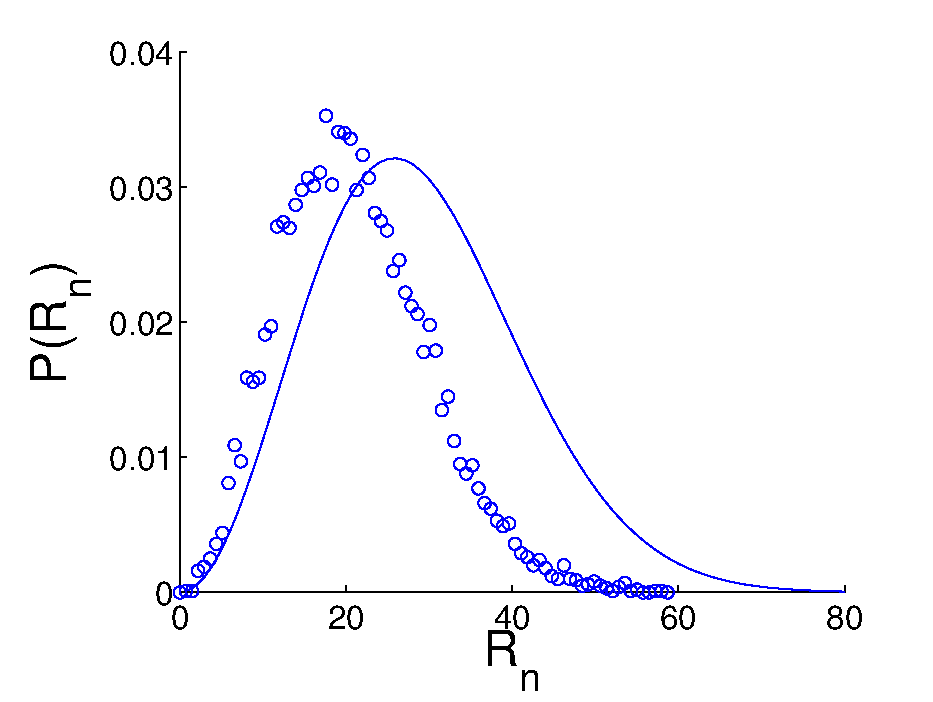
\includegraphics{binning-fcc-1000n-10ktr-80bin} % requires the graphicx package
   \caption{Probability distribution of simulated end-to-end distances for random walk in FCC lattice (empty circles) plotted against that of cubic lattice for comparison in clustering and spread behavior; done for n = 1000 steps, 10k trials, and 80 bins (solid line)}
   \label{fig:fccbinning}
\end{figure}

%--------------------------------------------------------------------------------------------------%

\end{document}  
